\documentclass[12pt, varwidth, border=5mm]{standalone}
\usepackage{tikz}
\usepackage{amsmath}
% Underlining package
\usepackage{ulem}
\usetikzlibrary{angles,quotes}
\usetikzlibrary{intersections}
\usetikzlibrary{arrows.meta}
\usetikzlibrary{calc}
% \usepackage[a4paper, portrait, margin=1cm]{geometry}


\begin{document}
\section*{ }
    
$\text{g} = \text{66}^\circ$
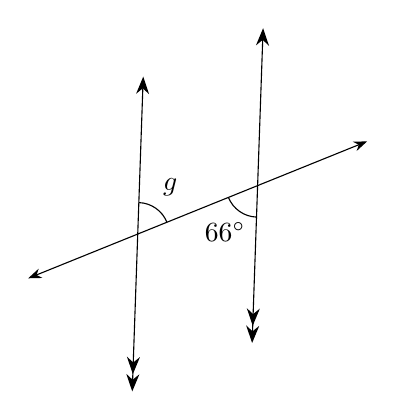
\begin{tikzpicture}[scale=1.0, baseline=(current bounding box.north)]
  \begin{scope}[rotate=202]
    % Draw the first line
    \draw[<->>, >={Stealth[scale=1.3]}, name path=P1] (0, 0) -- (1.6269465723032008, 3.6541818305704035);
    % Draw the second line with the calculated offsets
    \draw[<->>, >={Stealth[scale=1.3]}, name path=P2] (1.6419544177590701, 0) -- (3.2689009900622708, 3.6541818305704035);
    % Draw the transversal through the middle of the parallel lines
    \draw[<->, >=Stealth, name path=P3] (-0.6865267138483997, 1.8270909152852017) -- (3.9554277039106704, 1.8270909152852017);
    \path [name intersections={of=P1 and P3,by=A}];
    \path [name intersections={of=P2 and P3,by=B}];
    % Draw the angle
    \coordinate (p1s) at (0, 0);
    \coordinate (p1e) at (1.6269465723032008, 3.6541818305704035);
    \coordinate (p2s) at (1.6419544177590701, 0);
    \coordinate (p2e) at (3.2689009900622708, 3.6541818305704035);
    \coordinate (ts) at (-0.6865267138483997, 1.8270909152852017);
    \coordinate (te) at (3.9554277039106704, 1.8270909152852017);
    \draw pic["$g$", draw=black, -, angle eccentricity=1.8, angle radius=0.4cm] {angle=ts--B--p2s};
\draw pic["$66^\circ$", draw=black, -, angle eccentricity=1.8, angle radius=0.4cm] {angle=te--A--p1e};

  \end{scope}
\end{tikzpicture}

\end{document}
